\documentclass[12pt, letter paper]{article}
\usepackage[utf8]{inputenc}
\title{Manuscript}
\author{Rasmus Raschke}
\date{April 2026}
\usepackage{amsmath, amstext, amssymb} 
\usepackage{bm}
\usepackage{graphicx}
\usepackage[table,xcdraw]{xcolor} 
\usepackage{float}
\usepackage{siunitx}
\DeclareMathOperator{\SO}{SO}
\DeclareMathOperator{\so}{\mathfrak{so}}
\DeclareMathOperator{\sgn}{sgn}
\DeclareMathOperator{\grad}{grad}
\DeclareMathOperator{\Id}{id}
\usepackage[
    backend=biber,
    style=numeric,
    natbib=true,
    url=false, 
    doi=true,
    eprint=false,
    sorting=none,
]{biblatex}
\addbibresource{bibliography.bib}
\begin{document}
\section{Introduction}
TBD
\section{Equations of Motion}
\subsection{Analytical Derivation}
Consider a ball of radius $R$ and mass $M$ rolling without slipping on a plane
\begin{equation}
    \label{eq:hypersurface}
    H_\alpha := \{ (x,y,z) \in \mathbb{R}^3 \mid F:=z-\alpha y =0 \}\subseteq \mathbb{R}^3
\end{equation}
of slope $\alpha$ and unit normal field $\bm{n}:=\frac{\grad F}{\|\grad F\|}$.
Assume that the sphere carries a dipole moment $\bm{\mu}_0$ interacting with a homogeneous, constant magnetic field $\bm{B}$. The configuration manifold is \[
Q := H_\alpha \times \SO(3) \subseteq \mathbb{R}^3 \times \SO(3)
,\] where $\SO(3)$ is the three-dimensional special orthogonal Lie group. The velocity phase space is thus given by \[
TQ = TH_\alpha \times T\SO(3) \cong TH_\alpha \times \so(3) \cong \mathbb{R}^2 \times \mathbb{R}^3 \subseteq \mathbb{R}^6,
\] where $T$ denotes the tangent bundle and $\so(3)$ is the Lie algebra of $\SO(3)$. We choose the trivial global chart on $\mathbb{R}^3$ and some local smooth chart $\phi: U \subseteq \SO(3) \to \mathbb{R}^3$ on $\SO(3)$.\footnote{Constraining the motion to $H_\alpha$ reduces the system by one dimension, but we choose not to eliminate the $z$ coordinate since we need the solution in the full frame for numerical analysis.} A motion is a function \[
(\bm{r}(t), P(t)): \mathbb{R} \supseteq I \to \mathbb{R}^3 \times \SO(3),
\] where $\bm{r}(t)$ is a path in $\mathbb{R}^3$ and $P(t)$ is a path in $\SO(3)$, i.e., a time-parametrized special orthogonal matrix. Define $\bm{\theta}:= \phi \circ P: I \to \mathbb{R}^3$. Our goal is to find equations of motion and their solutions \[
(\bm{r}(t),\bm{\theta}(t))=(x(t),y(t),z(t),\theta_x(t),\theta_y(t),\theta_z(t)): I \to \mathbb{R}^6
\] in local coordinates. Using the canonical Euclidean basis $\mathcal{B}:=(\bm{e}_x,\bm{e}_y, \bm{e}_z)$, we define a non-moving (inertial) coordinate frame by choosing an arbitrary origin. Furthermore, we consider a rotating coodinate frame defined by $\hat{\mathcal{B}}(t):=P(t)\mathcal{B}$. The angular velocity in the inertial frame $\bm{\Omega}(t)=(\Omega_x, \Omega_y, \Omega_z)^\top$ is defined in terms of the cross product matrix $$\Omega^\times(t) = \dot{P}(t)P^\top(t) = 
\begin{pmatrix}
    0 & -\Omega_z & \Omega_y \\
    \Omega_z & 0 & -\Omega_x \\
    -\Omega_y & \Omega_x & 0
\end{pmatrix}
.$$ 
\begin{figure}[H]
\centering

\includegraphics[width=0.75\textwidth]{ramp.pdf}
\caption{Sketch of the system in the $yz$-plane. The hat vectors are vectors of the basis $\hat{\mathcal{B}}$ while vectors without hat refer to $\mathcal{B}$. Red vectors are projected and may have non-zero $\bm{e}_x$-components. The plane $H_\alpha$ has an angle of inclination $\varphi$ defined by $\alpha = \tan \varphi$. The outer magnetic field is kept fixed parallel to $\bm{e}_z$.}
\end{figure}
The kinetic energy form is given by 
\begin{equation}
    \label{eq:kinetic}
    T(\bm{r},\bm{\Omega})=\frac{M}{2}\|\dot{\bm{r}}\|^2 + \frac{I_0}{2}\|\bm{\Omega}\|^2
\end{equation}
and the potential by
\begin{equation}
    \label{eq:potential}
    U(z, \bm{\Omega})=-Mgz+\langle \hat{\bm{\mu}}(t), \bm{B}\rangle,
\end{equation}
where $\hat{\bm{\mu}}(t):=P(t)\bm{\mu}_0$, $I_0$ is the inertia scalar of an ideal ball, and $g$ is the gravitational acceleration. We obtain a Lagrangian $L(z,\bm{\Omega},\dot{\bm{r}}) := T - U$ and follow \cite{Bloch2015} for non-holonomic systems. Assuming that there is an external force $\bm{F}_\text{e}=\bm{F}_\text{e}(\bm{r})$ such as friction, the corresponding Lagrange-d'Alembert principle reads\cite{Crepel2005, Lagrange1788}
\begin{equation}
    \label{eq:lagrangealembert}
    \delta \int_0^t L(z(s),\bm{\Omega}(s), \dot{\bm{r}}(s)) \, ds + \int_0^t \langle \bm{F}_\text{e}(\bm{r}(s)), \delta \bm{r}(s)  \rangle \, ds=0 
    .\end{equation} The torque can be written as \[
\bm{\tau}= \bm{\tau}_\text{em} + \bm{\tau}_\text{e}
\] where $\bm{\tau}_\text{em}:=\hat{\bm{\mu}}(t) \times \bm{B}$ is the magnetic torque, and $\bm{\tau}_\text{e} := -R \bm{n} \times \bm{F}_\text{e}$ is the torque induced by external forces.
The phase space of the linear motion admits an orthogonal decomposition $\mathbb{R}^3 \cong H_\| \oplus H_\perp$ with respect to the normal $\bm{n}$. Thus we can decompose arbitrary $\bm{v} \in \mathbb{R}^3$ as $\bm{v}=\bm{v}_\| + v_\perp \bm{n}$.
With the rolling constraint
\begin{equation}
    \label{eq:rollingconst}
    \dot{\bm{r}} = R \bm{\Omega} \times \bm{n},
\end{equation}
integration by parts, and non-degeneracy of the scalar product, one obtains tangential 
\begin{equation}
    \label{eq:tangangularvel}
    \frac{d \bm{\Omega}_\|}{dt} = \frac{1}{I_0+MR^2} \bm{\tau}_\| - \frac{RMg}{I_0+MR^2}(\bm{n} \times \bm{e}_z) 
\end{equation}
and normal 
\begin{equation}
    \label{eq:normalangularvel}
    \frac{d \Omega_\perp}{dt} = \frac{\tau_\perp}{I_0}
\end{equation}
equations for the angular acceleration from Equation \ref{eq:lagrangealembert}. Taking the derivative of Equation \ref{eq:rollingconst}, this fully determines the linear motion. Assuming Coulomb friction and aerodynamical drag by the drag equation, the external force becomes \begin{equation}
    \label{eq:friction}
    \bm{F}_\text{e} = - \nu_\text{r} Mg \langle \bm{n},\bm{e}_z\rangle \sgn (\dot{\bm{r}}) + \frac{\rho C A}{2} \|\dot{\bm{r}}\|^2
    ,\end{equation} where $\nu_\text{r}$ is the rolling resistance coefficient, $\sgn$ is the sign function, $\rho$ is the fluid density of air, $C$ is the drag coefficient, and $A$ is the cross-sectional area of the sphere\cite{Coulomb, Hayakawa2005, Landau2002}. For numerical reasons, we reparametrize $P(t)=P((q_0(t),\bm{q}(t)))$, where \[
(q_0(t), \bm{q}(t)): I \to \mathbb{S}^3
\] is a time-dependent unit quaternion. Subsuming, the full eqations of motion are:
\begin{equation}
    \label{eq:eom}
    \begin{aligned}
        \frac{d^2 \bm{r}}{dt^2}&= \frac{5}{7M} \bm{\tau} \times \bm{n} - \frac{5g}{7} (\bm{e}_z)_\|, \\
        \frac{d\bm{\Omega}_\|}{dt} &= \frac{5}{7MR^2}\bm{\tau}_\| - \frac{5g}{7R} \bm{n} \times \bm{e}_z,\\
        \frac{d \Omega_\perp}{dt} &= \frac{5}{7MR^2} \tau_\perp, \\
        \frac{d(q_0,\bm{q})}{dt}&=\frac{1}{2}(0, \bm{\Omega}) \cdot (q_0, \bm{q}).
\end{aligned}
\end{equation}
\subsection{Numerical Solution}
The equations of motion were solved with our program $\mathtt{magsphere}$\cite{magsphere2026}. We implemented a Runge-Kutta-Munthe-Kaas-4 method, combining the quaternion-adapted Munthe-Kaas integrator with the Runge-Kutta 4 algorithm\cite{Butcher1996, MuntheKaas1998}. To avoid numerical instability at the discontinuities in Equation \ref{eq:friction}, we approximated \[
    \sgn(\dot{\bm{r}}) \approx \tanh(k \| \dot{\bm{r}}\|)
,\] where $k$ is a dimensionless constant describing the steepness of $\tanh$ around the origin. For the rolling resistance coefficient, we estimated $\nu_\text{r}=0.002$ based on values of $\nu_\text{r}$ for tires on steel and rubber surfaces\cite{Guba2023}.
Assuming the International Standard Atmosphere and moderate velocities, values of $\rho = 1.2 \, \unit{kg.m^{-3}}$ and $C=0.47$ were used for simulations\cite{iso2533, Baker1983}.
\section{Results}
\subsection{Influence of the magnetic moment}
\begin{figure}[H]
    \centering
    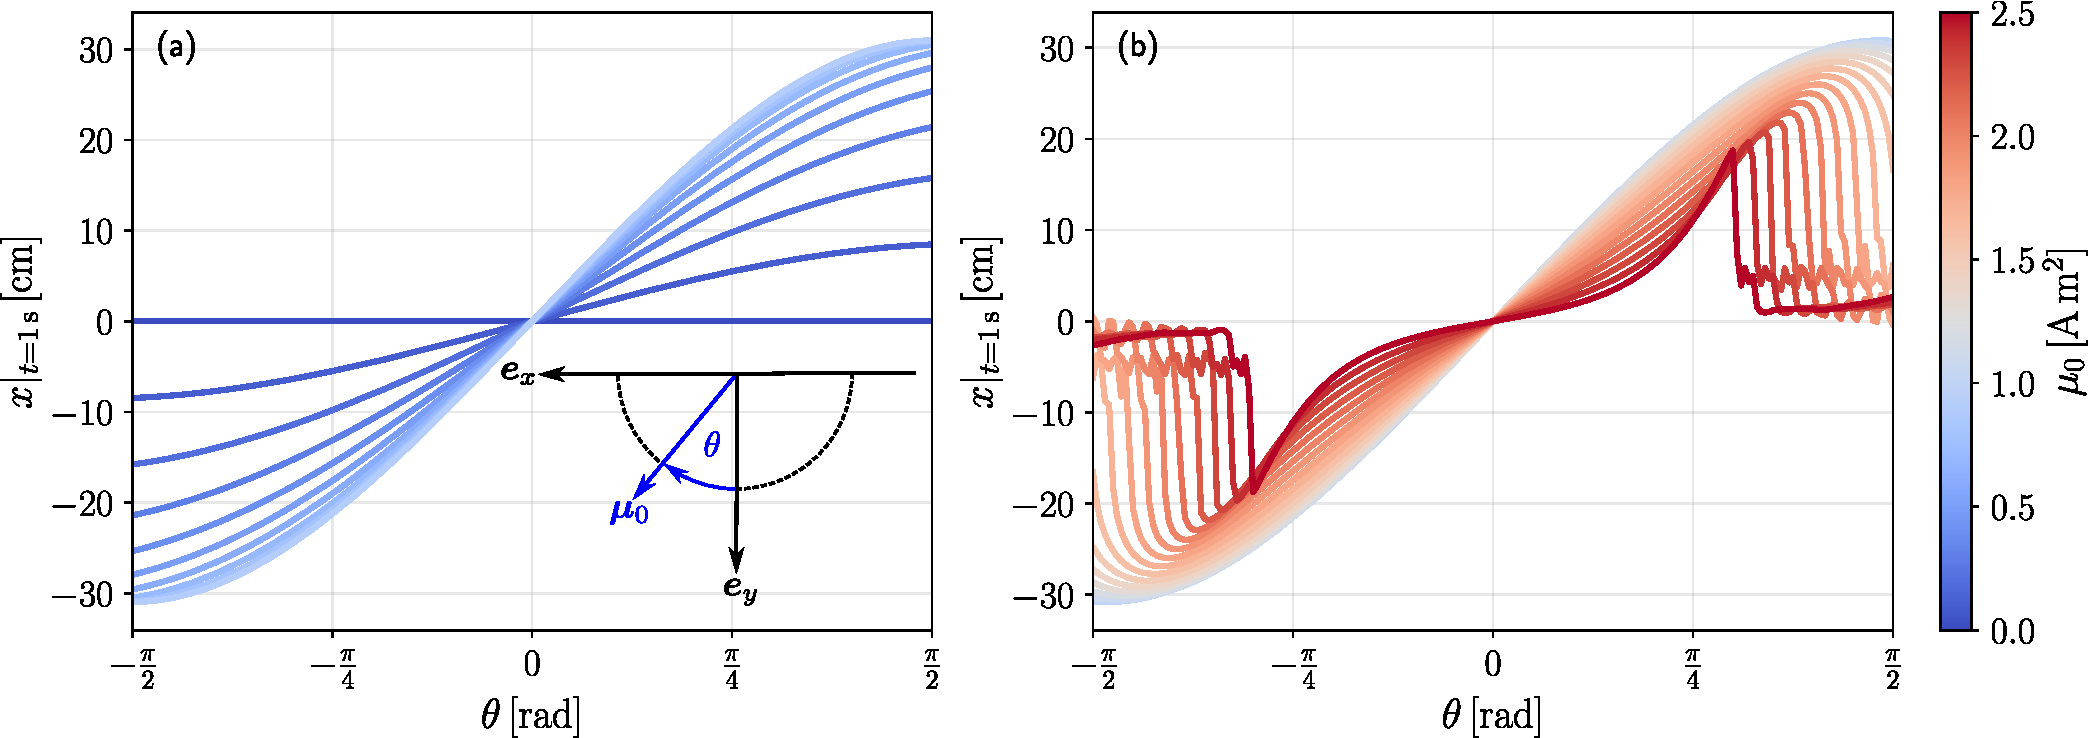
\includegraphics[width=\textwidth]{f1.pdf}
    \caption{Final deviation $x|_{t=1 \, \unit{s}}$ in relation to angle $\theta$ and modulus $\mu_0$. Each graph is associated with a fixed modulus $\mu_0$, where (a) shows curves for moduli below $1 \, \unit{\ampere\per\metre\squared}$ and (b) for moduli including and above $1 \, \unit{\ampere\per\metre\squared}$. In the small $\mu_0$-regime (a), the final derviation increases in magnitude with $\theta$ and is antisymmetric around the origin. The high $\mu_0$-regime (b) displays similar antisymmetry, yet different behaviour for high magnitudes of $\theta$. With increasing modulus, critical points shift towards lower absolute values of $\theta$, after which the curves behave erratic.}
    \label{fig:f1}
\end{figure}
\begin{figure}[H]
    \centering
    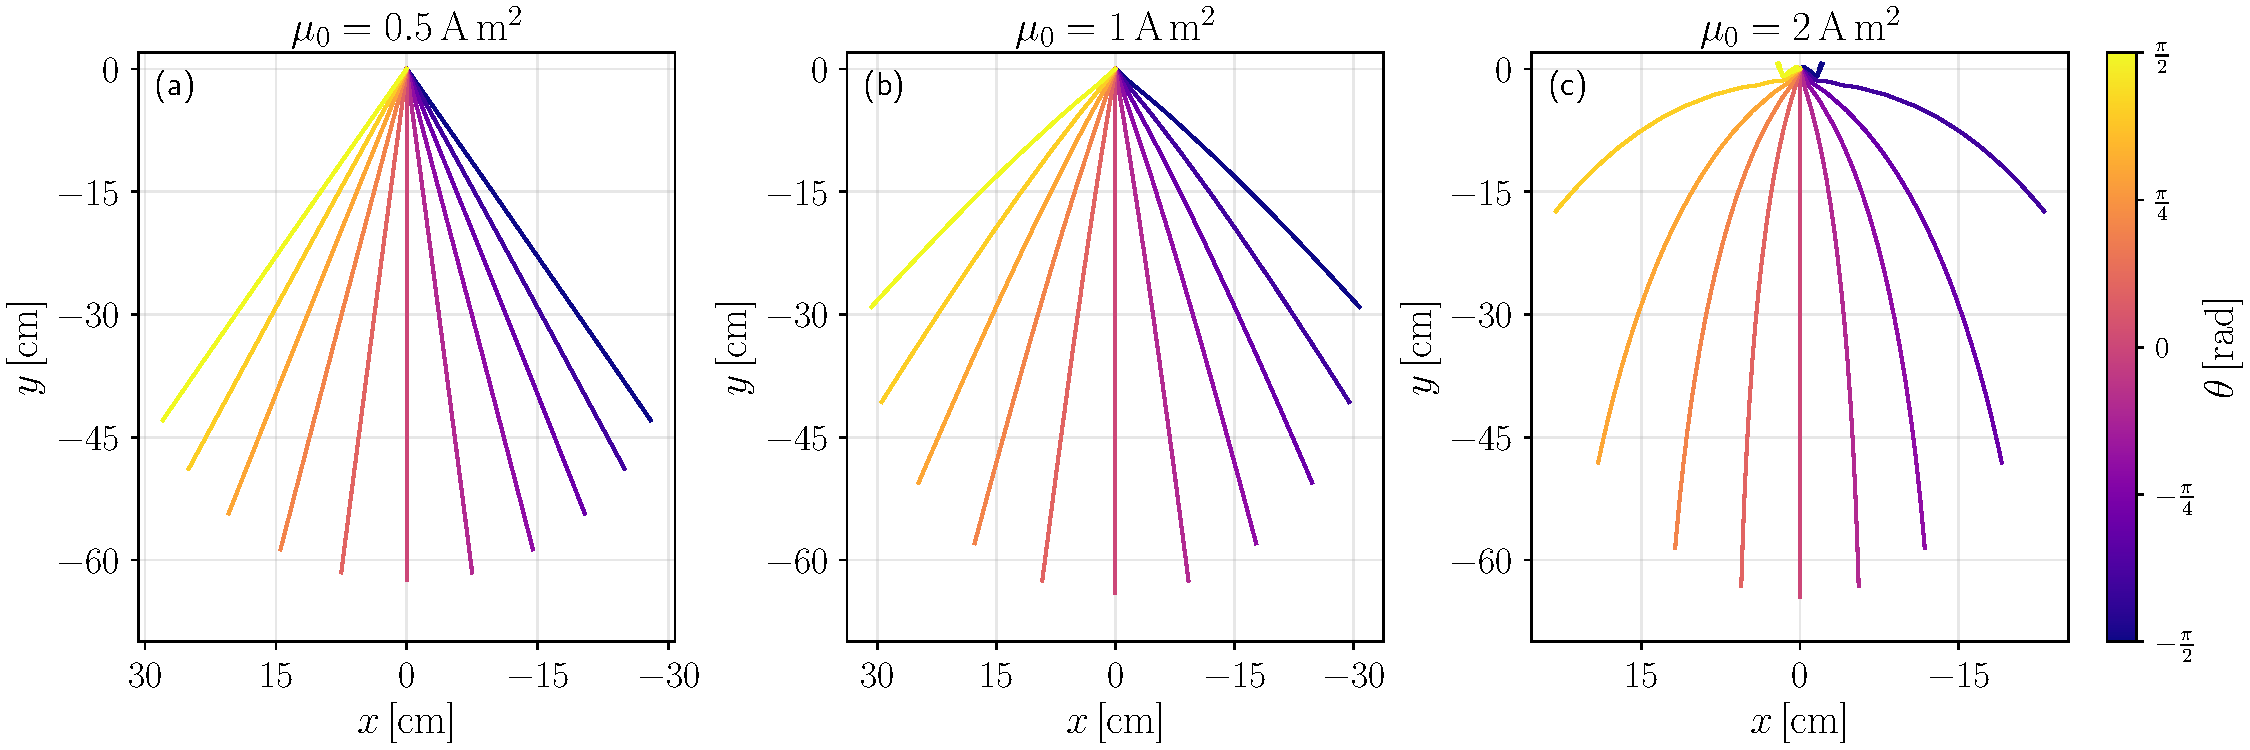
\includegraphics[width=\textwidth]{f2.pdf}
    \caption{Trajectories on the $xy$-plane for selected moduli. The outward curvature of the trajectories increases with $|\theta|$ and $\mu_0$, as anticipated. Note that in the high-modulus regime (c), the two outmost trajectories loop in on themselves as the magnetic force overcompensates the gravitational force.}
    \label{fig:f2}
\end{figure}
We investigated the influence of the initial magnetic moment vector $\bm{\mu}_0$ on the trajectories for an incline angle of $\varphi = 10^\circ$. Firstly focussing on the influence of the deviation of $\bm{\mu}_0$ from the plane spanned by $\bm{B}$ and the downhill direction, we parametrized \[
    \bm{\mu}_0 = \mu_0 (\sin \theta, \cos \theta, 0)^\top
\]  with $\mu_0 := \|\bm{\mu}_0\|$ and an angle $\theta$ defined as depicted in Figure \ref{fig:f1}. We chose the value of the $x$-coordinate after one second as measure for the deviation of the actual trajectory from a straight downhill path. The results are also shown in Figure \ref{fig:f1}. Antisymmetric behaviour in $\theta$ is predicted by $\bm{\mu}(-\theta)=-\bm{\mu}(\theta).$ The deviation from the straight path grows non-linearly with $\mu_0$, saturating in the low-modulus regime while reaching an extremum in the high-modulus regime. Figure \ref{fig:f2} shows that the increasing curvature of the trajectories reduces their total length, corresponding to the saturation of $x$-deviation. In the high-modulus regime, the magnetic force can dominate over gravity, causing the paths to trace out loops. This explains the observed erratic behaviour beyond the global extrema in Figure \ref{fig:f1}(b).\newline
Secondly, we parametrized \[
    \bm{\mu}_0=\mu_0(0, \sin \psi, \cos \psi)^\top
\] to investigate the influence of the $xz$-deviation of $\bm{\mu}_0$. The measure for the influence is the $y$-coordinate after one second as there is no $x$-deviation when $\bm{\mu}_0$ and $\bm{B}$ align in the $yz$-plane.
\begin{figure}[H]
    \centering
    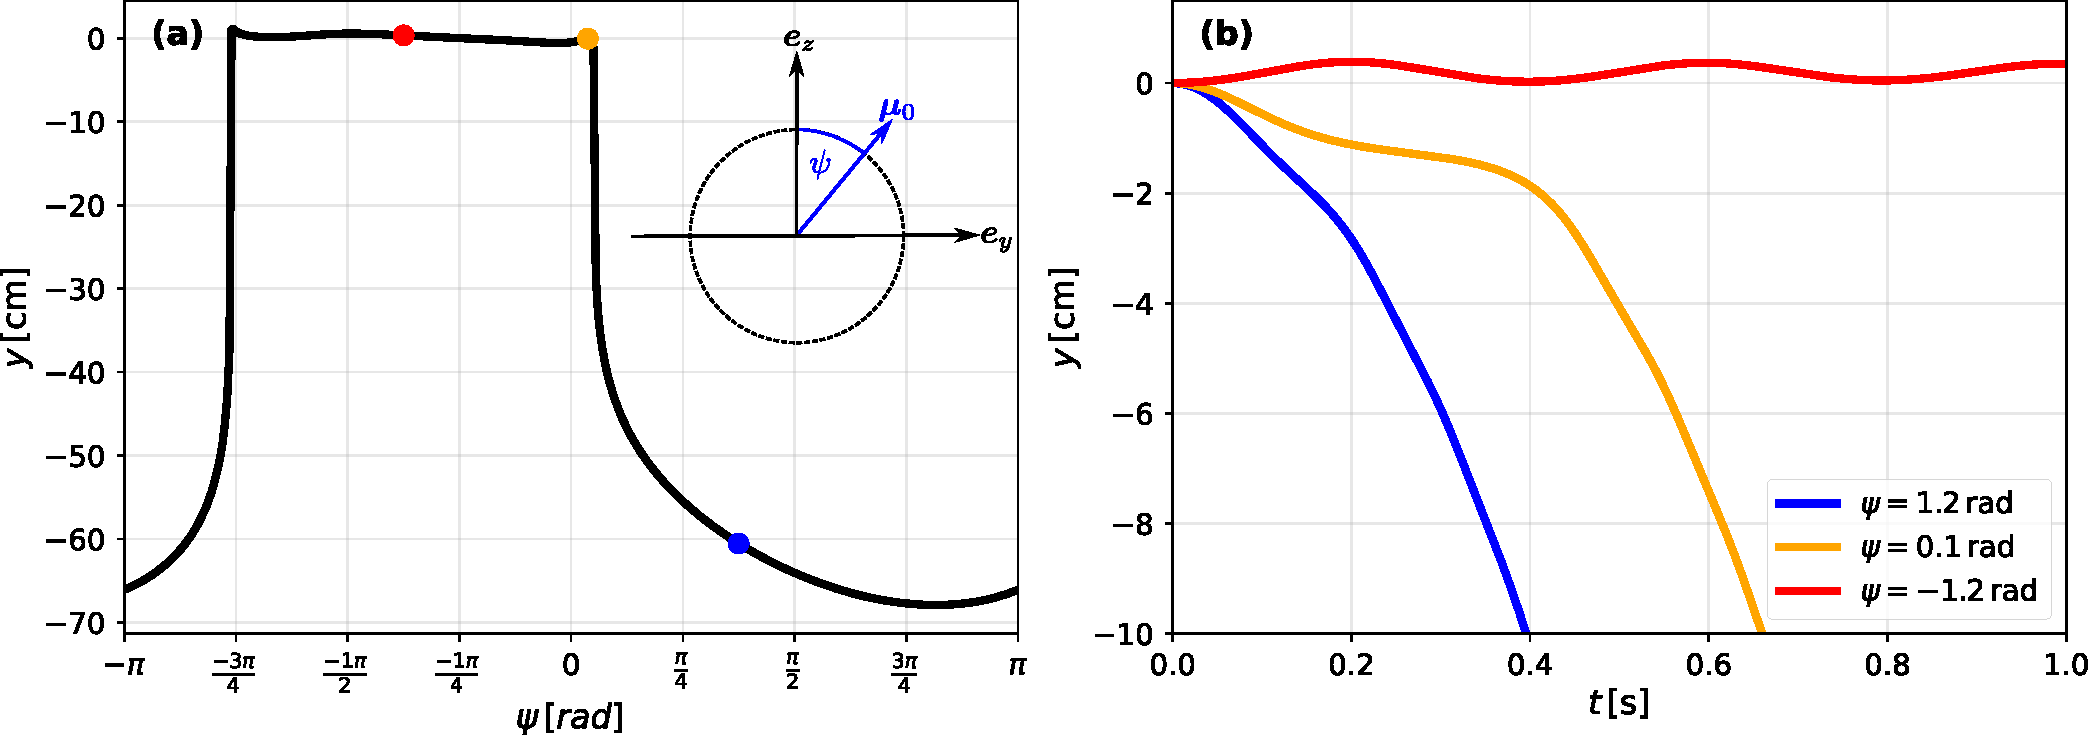
\includegraphics[width=\textwidth]{g.pdf}
    \caption{Final $y$-distance in relation to angle $\psi$; $y(t)$-coordinate in relation to time. Figure (a) shows three different regimes: a high-deviation regime, a low-deviation regime, and an intermediate regime. For each one of these, a representative $y$-trajectory is shown in (b). The low-deviation regime (blue) corresponds to a gravity-dominated downhill trajectory, the high-deviation regime (red) to a magnetic-dominated oscillatory trajectory, and the intermediate regime (orange) to a path where gravity dominates only after initial oscilltory behaviour.}
    \label{fig:g}
\end{figure}
Figure \ref{fig:g} clearly shows that for angles between about $\frac{-3\pi}{4}\, \unit{rad}$ and $0 \, \unit{rad}$, the magnetic force fully dominates over the gravitational force, thus the ball oscillates in the $yz$-plane without rolling down. This behaviour transitions to oscillations which are eventually overcome by gravity at a specific point in time. The more favourable the downhill motion is for the total magnetic energy, the sooner the critial point is reached.
\section{References}
\printbibliography[heading=none]
\end{document}
